\chapter{Numerical results}
\label{chap:results}

\prettyref{chap:patching} and \prettyref{chap:MPOcontr} introduced our \emph{patched QTCI} and \emph{patched MPO–MPO contraction} algorithms in detail. By extending the state-of-the-art implementation of the QTCI algorithm, we have implemented a \textit{divide‐and‐conquer} version of TCI that targets scenarios in which the standard routine may struggle.

In this chapter we first present representative benchmarks (\prettyref{sec:2DGreen} and \prettyref{sec:benchmarkMPOMPOContr}) that highlight the performance of the new routines. We then apply them to two physics problems that have previously posed computational bottlenecks: the computation of the bare susceptibility for the 2D Hubbard model with momentum dependence (\prettyref{sec:bubbleCalc}) and vertex contractions during the solution of the Bethe-Salpeter for the single‐impurity Anderson model (Sec.~\ref{sec:patchBSE}). Both cases were recently addressed with QTCI or patched quantics SVD–based tensor trains approaches \cite{Hiroshi2023,Rohshap2025}. Our patched QTCI method complements and extends those efforts, demonstrating improved efficiency on the same benchmark tasks.

Our calculations are constructed on the already mature $\julia$ packages \texttt{TensorCrossInterpolation.jl} \cite{TensorCrossInterpolation.jl} and \texttt{QuanticsTCI.jl} \cite{tensor4all.org}, which we have extended with the additional features required for the present patched applications.

\section{Approximation of 2D Green's functions}
\label{sec:2DGreen}

We begin with the toy Green’s function  

\begin{equation}
  G(\mathbf{k})
  \;=\;
  \frac{1}
       {\;\omega+\mu-\varepsilon_{\mathbf{k}}+i\delta\,},
  \label{eq:2DGreen}
\end{equation}

where the non-interacting dispersion is taken as
\(\varepsilon_{\mathbf{k}}=-2\cos k_{x}-2\cos k_{y}\)  
and we set the chemical potential to \(\mu=0\).
\prettyref{eq:2DGreen} is patterned after the Matsubara Green’s function of the two-dimensional Hubbard model at finite temperature
\cite{Mahan2000},

\begin{equation}
  G(\bk,i\nu)
  \;=\;
  \frac{1}
       {\,i\nu+\mu-\varepsilon_{\mathbf{k}}-\Sigma(\bk,i\nu)},
\end{equation}

with two deliberate simplifications:
\(\omega\) plays the role of the (real) self-energy
\(\Sigma\), while \(\delta\) mimics the Matsubara frequency
\(\nu=(2n+\xi)\pi/\beta\) ($\xi=0,1$ for bosons and fermions) and thus encodes the temperature.
Accordingly we treat \(\omega\) as a fixed input—one may think of it as the self-energy obtained from the previous Dyson iteration—whereas \(\delta\) is varied to emulate different temperatures.

The figure below shows a density plot of
\(\operatorname{Re}G(\mathbf{k})\) for the representative choice
\(\omega=10^{-1}\):

\begin{figure}[ht!]
    \centering
    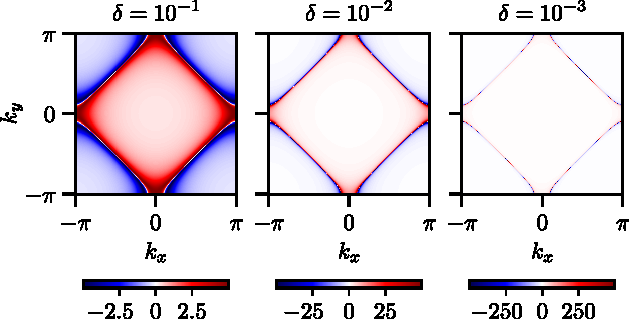
\includegraphics{figures/realGreenHeatmap.pdf}
    \caption{Heatmap of the real part of the Green's function in \prettyref{eq:2DGreen}, $\text{Re}\left(G(\bk)\right)$ for different values of $\delta$ and fixed $\omega=10^{-1}$. }
    \label{fig:realGreenHeatmap}
\end{figure}

\prettyref{fig:realGreenHeatmap} shows that the parameter \(\delta\) controls how sharply the Green’s function is localised: as \(\delta\to 0\) the poles narrow and \(G(\mathbf{k})\) becomes increasingly singular.  This makes the function an ideal testbed for patched QTCI.

We discretise \(G(\mathbf{k})\) by quantics rebasing,  
\begin{equation}
  G(\bk)
  \;\longrightarrow\;
  G_{\bsigma} = G \bigl(\bk(\bsigma)\bigr),
\end{equation}
with bit string
\(\boldsymbol{\sigma}=(\sigma_{1},\dots,\sigma_{\mathcal R})\) in the fused
ordering, or \(\boldsymbol{\sigma}=(\sigma_{x1},\dots,\sigma_{y\mathcal R})\) in the interleaved ordering.  
Throughout we use \(\mathcal R=15\) bits per \(\bk\)-component.

After setting a patch bond–dimension cap \(\chi_{\text{patch}}\) and a global tolerance \(\tau=10^{-7}\), we monitor convergence of pQTCI via the pointwise error
\begin{equation}
  \varepsilon(\mathbf{k})
  = \log_{10}\!
      \frac{\bigl|\operatorname{Re}\widetilde G(\mathbf{k})
                -\operatorname{Re}G(\mathbf{k})\bigr|}
           {\;\|\operatorname{Re}\widetilde G\|_{\infty}},
  \label{eq:localError2DGreen}
\end{equation}
where \(\|\operatorname{Re}\widetilde G\|_{\infty}\) is the maximum of \(|\operatorname{Re}\widetilde G|\) over all sampling points \(\bk(\bsigma)\) used in every patch \(\operatorname{Re} \widetilde{G}^{p_1,\dots,p_{\bar\ell}}\) produced by the patched QTCI routine.

\prettyref{fig:2DGreenErrorHeatmap} compares the patched QTCI approximation with the exact real part of the Green’s function for three values of the
broadening parameter \(\delta\).  The top row shows
\(\operatorname{Re}G(\bk)\) reconstructed from the patched tensor trains, while the bottom row plots the local error \(\varepsilon(\bk)\) defined in \prettyref{eq:localError2DGreen} over the entire Brillouin zone \([-\pi,\pi]^{2}\). To evaluate the approximate tensor
\(\operatorname{Re}\widetilde{G}_{\bsigma}\) on a uniform \(\bk\)-grid we first invert the mapping \(\bsigma\mapsto\bk(\bsigma)\) and then, after resumming the whole patches set $\text{Re}\bigl(\widetilde{G}^{p_1,\dots,p_{\ellb}}\bigr)$ to a single TT approximation $\text{Re}\bigl(\widetilde{G}_{\bsigma}^{+}\bigr)$, we evaluate the correspondent $\bsigma(\bk)$ tensor value for each $\bk$ point of the domain. \prettyref{fig:2DGreenErrorHeatmap}  also displays the bond–dimension distributions for both the patched and the single-TT approximations of \(\operatorname{Re}G(\bk)\)  at the three caps $\chip=48,118,277$ (corresponding to  $\delta=10^{-1},10^{-2},10^{-3}$). The patches shows a marked rank reduction compared to the QTCI TT. Moreover we can distiguish two patch groupings: large, low-rank patches span the ``trivial'' regions of the Brillouin zone, while smaller patches—carrying the higher bond dimensions—track the non-trivial, sharply structured areas. The bond dimensions in show this patch separation.

\begin{figure}[htbp]
    \centering 
    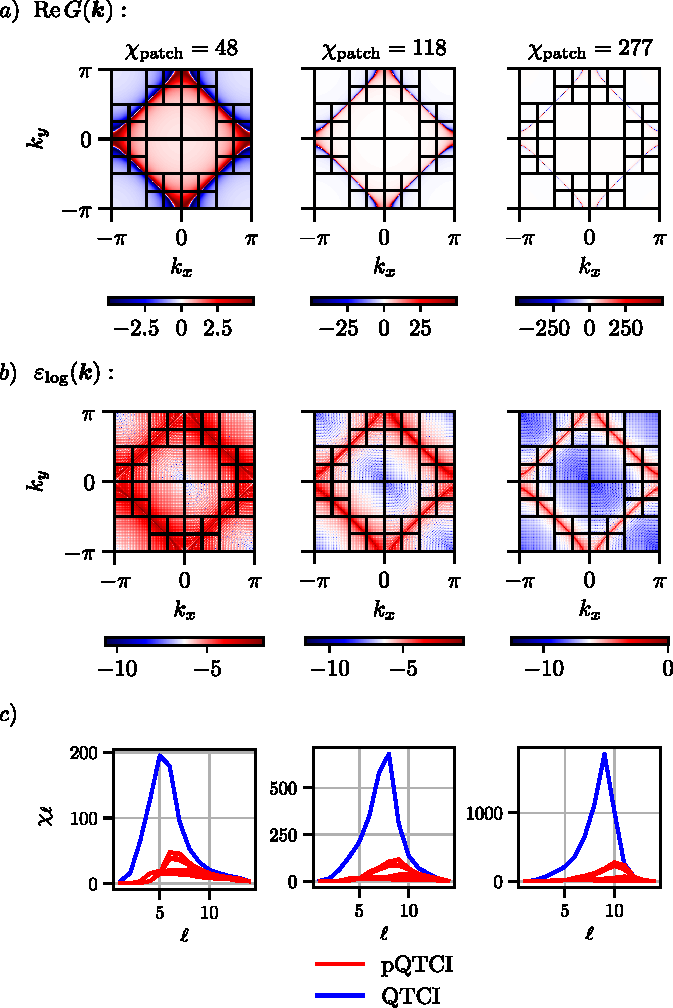
\includegraphics{figures/2DGreenErrorHeatmap.pdf}
    \caption{Patched QTCI approximation of
           \(\operatorname{Re}G(\bk)\).
           $(a)$ Heatmaps of the patched tensor train evaluated on \([-\pi,\pi]^{2}\) for bond–dimension caps \(\chi_{\text{patch}}=48,118,277\) (corresponding to
           \(\delta=10^{-1},10^{-2},10^{-3}\), respectively).
           $(b)$ Log–error \(\varepsilon(\bk)\) [\prettyref{eq:localError2DGreen}]
           for the same patched approximations. 
           $(c)$ Comparison of the bond-dimension profiles for the pQTCI and standard QTCI representations of \(\operatorname{Re}G(\bk)\). Every patch in the pQTCI result adheres to the prescribed cap $\chip$.}
    \label{fig:2DGreenErrorHeatmap}
\end{figure}
Despite the fact that \(\varepsilon(\bk)\) does not drop everywhere below the target tolerance \(\tau=10^{-7}\), its \emph{spatial average} error is of that
order. For the same parameters the conventional (Q)TCI routine attains comparable accuracy, as illustrated in \prettyref{fig:TCI2DGreenerror} for \(\delta=10^{-1}\).
\begin{figure}[htbp]
    \centering
    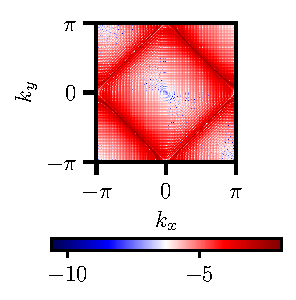
\includegraphics{figures/heatmap_TCI_error_2DGreen_ω_0.1_δ_0.1_R_15_abstol_1.0e-7_unfol_fused.pdf}
    \caption{Local error \(\varepsilon(\bk)\) for a standard QTCI approximation of \(\operatorname{Re}G(\bk)\) at \(\delta=10^{-1}\).}
    \label{fig:TCI2DGreenerror}
\end{figure}
A one–dimensional cut at \(k_{y}=\pi/2\) (\prettyref{fig:lineError2DGreen}) confirms that the patched approximation faithfully reproduces the sharp features of \(\operatorname{Re}G(\bk)\) for all three
\(\delta\) values.
\begin{figure}[htbp]
    \centering
    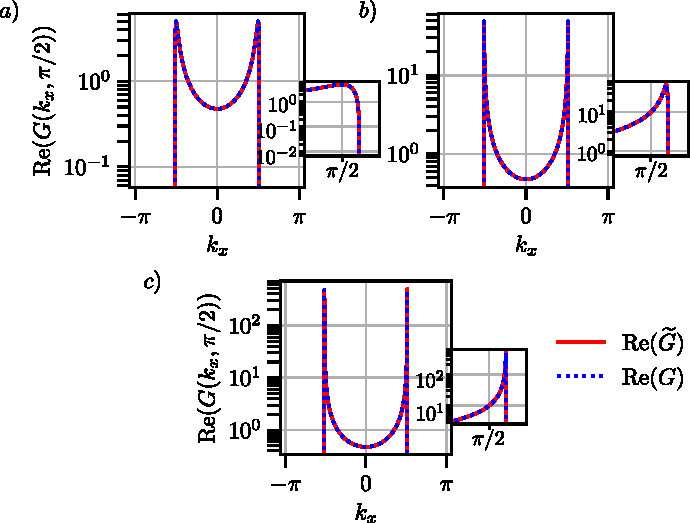
\includegraphics{figures/lineError2DGreen.pdf}
    \caption{One–dimensional slice,
           \(\operatorname{Re}G(k_{x},k_{y}=\pi/2)\),
           comparing the patched approximation (solid red) with the exact
           function (dotted blue) for
           \(\delta=10^{-1}\) (a),
           \(\delta=10^{-2}\) (b),
           and \(\delta=10^{-3}\) (c).}
    \label{fig:lineError2DGreen}
\end{figure}

We now benchmark patched QTCI (pQTCI) against the standard QTCI routine for
the Green’s function introduced above.  For each broadening
\(\delta\in\{10^{-1},10^{-2},10^{-3}\}\) we measure

\begin{itemize}
  \item the \emph{run time} on an Intel\textsuperscript{\textregistered}
        Xeon\textsuperscript{\textregistered} W-2245 CPU @ 3.90 GHz, and
  \item the \emph{memory footprint}, here defined as the total number of
        floating-point parameters in all patches
        \(\operatorname{Re}\widetilde{G}^{p_{1},\dots,p_{\bar\ell}}\).
\end{itemize}

The tensor \(\operatorname{Re}G_{\bsigma}\) is discretised with
\(\mathcal R=15\) bits per momentum component and approximated to a tolerance
\(\tau=10^{-7}\).  We scan the bond–dimension cap
\(\chi_{\text{patch}}\) and compare fused and interleaved bit orderings.

\begin{figure}[htbp]
    \centering
    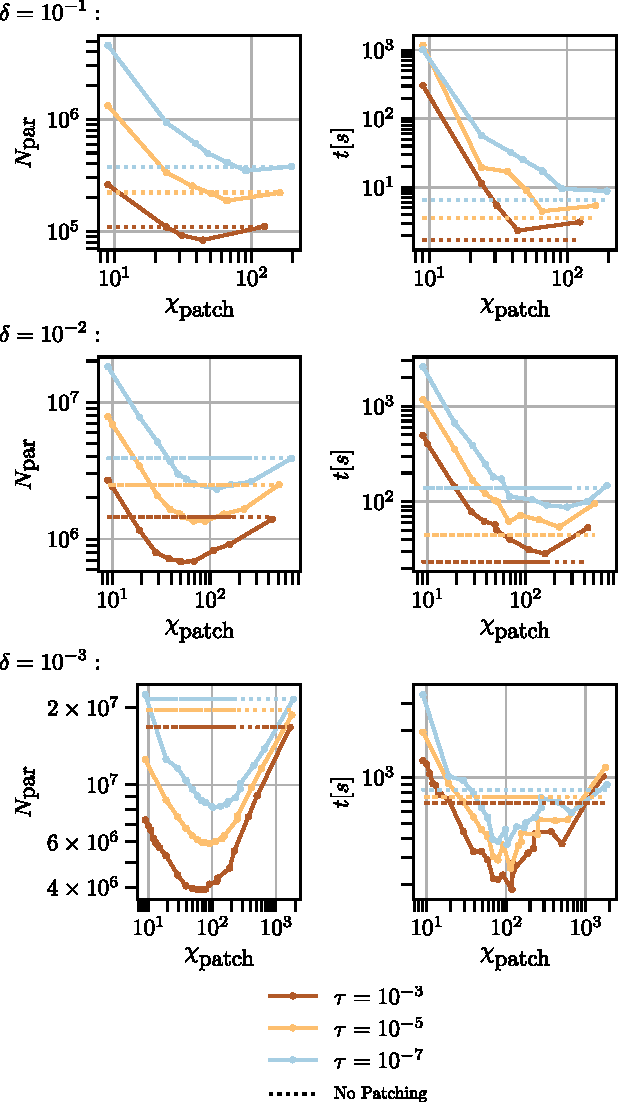
\includegraphics{figures/2DGreenMemoryTimeFused.pdf}
    \caption{ \textbf{Fused ordering.} Total parameter count (left) and CPU run time (right) versus bond-cap \(\chi_{\text{patch}}\) for \(\delta=10^{-1},10^{-2},10^{-3}\). Dotted lines show the corresponding standard-QTCI values. }
    \label{fig:memoryTime2DGreenFused}
\end{figure}

\begin{figure}[htbp]
    \centering
    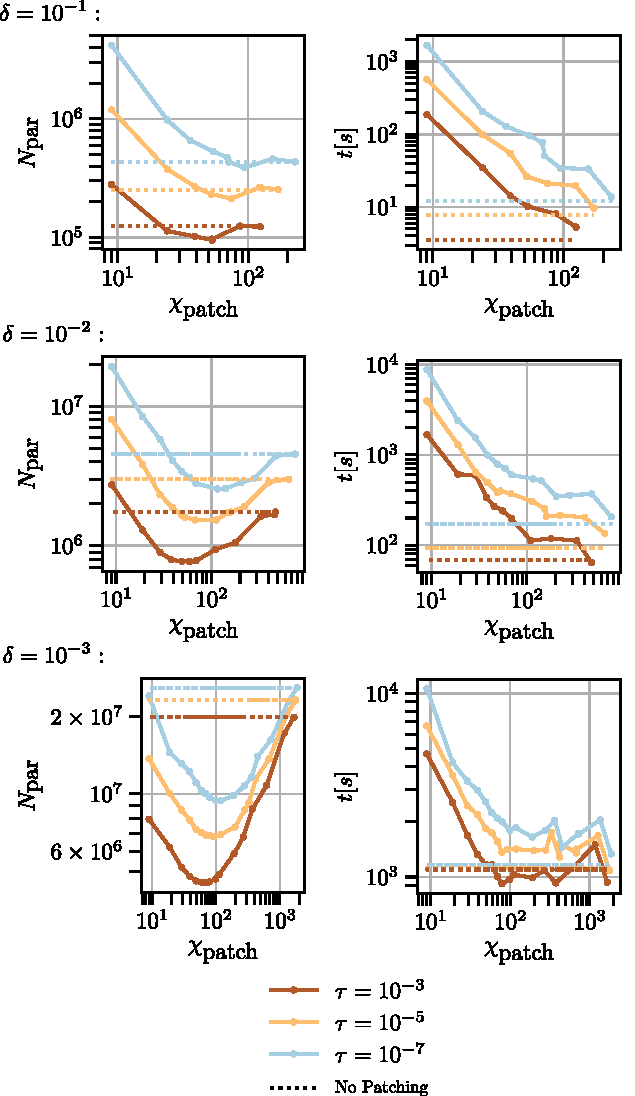
\includegraphics{figures/2DGreenMemoryTimeInterleaved.pdf}
    \caption{\textbf{Interleaved ordering.}
    Same data as \prettyref{fig:memoryTime2DGreenFused}, but with
    interleaved bit strings.}
    \label{fig:memoryTime2DGreenInterleaved}
\end{figure}

Figures~\ref{fig:memoryTime2DGreenFused}–
\ref{fig:memoryTime2DGreenInterleaved} reveal three main trends:

\begin{enumerate}
\item For \(\delta=10^{-2}\) and \(10^{-3}\) the patched routine beats standard QTCI in memory requirements. CPU rutime is smaller only with fused intex ordering. The advantage grows as the poles sharpen (smaller~\(\delta\)).

\item Each curve exhibits an optimal
      \(\chi_{\text{patch}}^{\mathrm{best}}\): setting the cap too low triggers the ``overpatching'' effect discussed in
      \prettyref{sec:patchingCost}, inflating the patch count without reducing ranks further.

\item Surprisingly, the fused ordering runtimes performs better than the interleaved one, although,in most cases, both respect the theoretical patch bounds of \prettyref{eq:chiPatchBound} for the total number of patches $\Np$. (cf. Sec.~\ref{app:2DGreenbounds} of \prettyref{app:bounds} for more details).
\end{enumerate}

For the broadest line, \(\delta=10^{-1}\), pQTCI offers no gain—the function is already smooth enough that a single TT suffices, and the extra slicing merely adds overhead.

A global view of the “return on investment’’ is given in \prettyref{fig:deltavsMemoryTime}, which plots the ratio of plain QTCI result to the best patched result (in parameters and run time) as a function of \(\delta\).  The larger is the ratio, the greater the benefit of using pQTCI.

\begin{figure}[htbp]
    \centering
    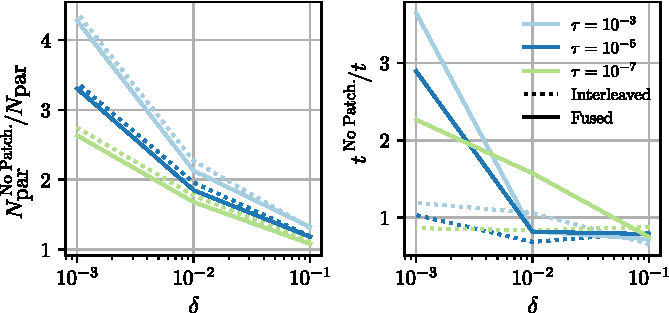
\includegraphics{figures/localisationParam2DGreen.pdf}
    \caption{Parameter and run-time ratios between the best patched approximation (at \(\chi_{\text{patch}}^{\mathrm{best}}\)) and a single-TT QTCI
    approximation, as a function of the broadening \(\delta\).} 
    \label{fig:deltavsMemoryTime}
\end{figure}

In summary, adaptively partitioning the domain allows one to focus bond dimension where it is truly needed, yielding significant savings for sharply localised Green’s functions, while incurring in overhead (``overpatching'') when the function is already smooth.

\section{Benchmarking of Patched MPO-MPO Contractions}
\label{sec:benchmarkMPOMPOContr}
Consider the two model functions 

\begin{align}
f(\bx) = \sum_{j=1}^4 e^{-(\bx - \bx_j)^2/\sigma^2_j}, \quad  
g(\bx) = \sum_{j=1}^4 e^{-|\bx - \bx'_j|/\sigma_j}, 
\label{eq:linearGauss}
\end{align}
with $\bx_j = (\cos \phi_j, \sin \phi_j )$, $\phi_j = (j-\frac{1}{2}) \frac{\pi}{2}$, $\sigma_j =  2^{-(j+1)}$, and $\bx'_j =\bx_j + (2\sigma_j,
\sigma_j)$. \prettyref{fig:factorsHeatmaps} shows heatmaps of \(f\) and \(g\).

\begin{figure}[htbp]
    \centering
    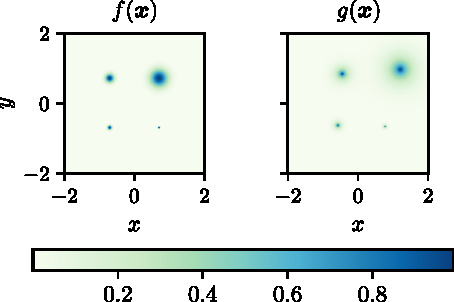
\includegraphics{figures/linearCombGauss.pdf}
    \caption{Heatmap of $f(\bx)$ and $g(\bx)$ defined in \prettyref{eq:linearGauss}.}
    \label{fig:factorsHeatmaps}
\end{figure}

We convert each function to a tensor via quantics rebasing (fused or interleaved),
\begin{equation}
    f(\bx) \mapsto \mF_{\bsigma}, \quad g(\bx) \mapsto \mG_{\bsigma}.
    \label{eq:tensorFactors}
\end{equation}
Applied to \(\mF_{\bsigma}\) and \(\mG_{\bsigma}\), the patched QTCI routine yields collections of tensor–train patches \(\{\mF^{p_{1},\dots,p_{\bar\ell}}_{\bsigma}\}\) and \(\{\mG^{p_{1},\dots,p_{\bar\ell}}_{\bsigma}\}\). We use these patch representations, after MPS-to-MPO folding (cf. \prettyref{eq:MPStoMPO}), as input for our \textit{patched MPO-MPO contraction} routines.

\subsection{Matrix multiplication}

Let the tensors \(\mF_{\bsigma}\) and \(\mG_{\bsigma}\) be stored in the \emph{interleaved} quantics format  

\[
  \bsigma
  =( \sigma_{x,1},\sigma_{y,1},\sigma_{x,2},\sigma_{y,2},\dots,
     \sigma_{x,\mathcal R},\sigma_{y,\mathcal R}),
  \qquad
  \mathcal R=17.
\]

When pQTCI is applied, the slicing (projection) order determines the resulting
patch tiling:
\begin{itemize}
  \item \textbf{Row patching:}\;
        \(p_{x,1}\!\to p_{x,2}\!\to\cdots\to p_{x,\mathcal R}\)
        (top–left panel of \prettyref{fig:patchingPatternsMatMul});
  \item \textbf{Column patching:}\;
        \(p_{y,1}\!\to p_{y,2}\!\to\cdots\to p_{y,\mathcal R}\)
        (centre–left panel);
  \item \textbf{Interleaved patching:}\;
        \(p_{x,1}\!\to p_{y,1}\!\to p_{x,2}\!\to\cdots\to p_{x,\mathcal R}\)
        (bottom–left panel).
\end{itemize}

Because pQTCI is adaptive, the actual patch pattern follows the feature structure of the functions; from left to right, each column in \prettyref{fig:patchingPatternsMatMul} correspond to the factors in \prettyref{eq:linearGauss} and their patched MPO contraction, respectively.

Each tensor‐train patch can be folded into an MPO (\prettyref{eq:MPStoMPO}) and fed to the patched MPO–MPO contraction routines.  
For instance, the two–dimensional convolution  
\begin{equation}
    h(x,y) = \int ds f(x,s)s(x,s)
\end{equation}
maps to the patched ``matrix multiplication'' 

\begin{equation}
    \mathcal{H}_{\bsigma\bsigma''} = \sum_{\bsigma'} \mF_{\bsigma\bsigma'}\mG_{\bsigma'\bsigma''},
    \label{eq:matrixMulTensors}
\end{equation}

where only mutually compatible patch pairs need be multiplied. Although the labels “row”  and “column” may seem inverted when viewed against the two-dimensional tilings in \prettyref{fig:patchingPatternsMatMul}, they are perfectly natural in the \emph{matrix} interpretation of each tensor—where the 
$x$-bit string forms the row index and the 
$y$-bit string the row index.

\begin{figure}[htbp]
    \centering
    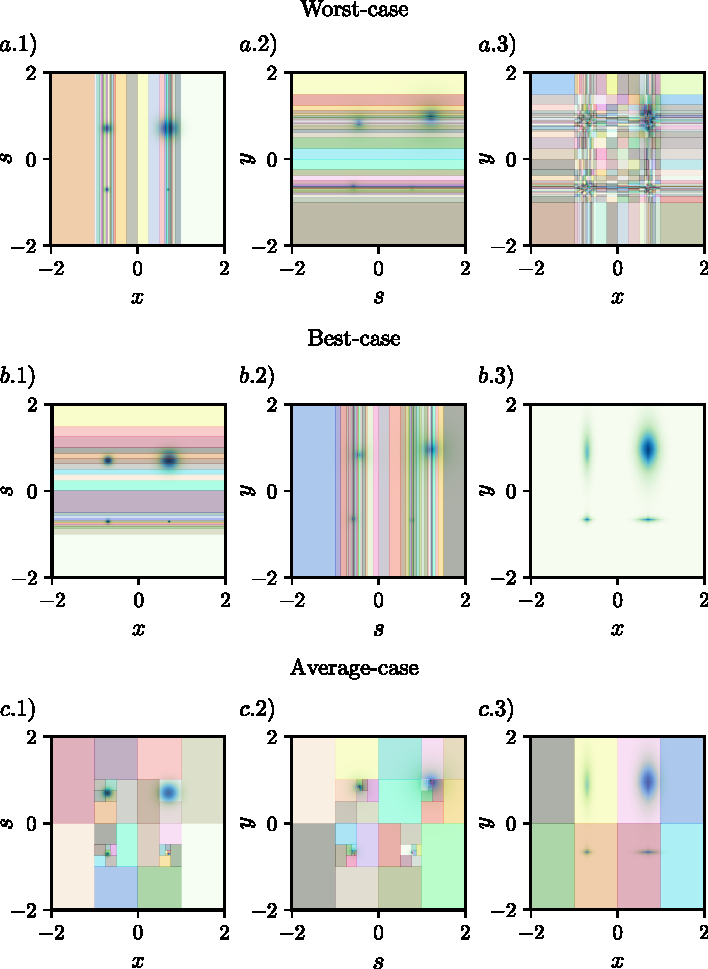
\includegraphics{figures/PatchContrResults.pdf}
    \caption{Patch tilings for the two factors \(\mF\) (panels
    $a-c.1$) and \(\mG\) $(a-c.2)$, together with the corresponding
    patched product \(\mathcal H\) $(a-c.3)$. Rows illustrate three representative patching contraction strategies as in \prettyref{fig:2DPatchMatMul}: $(a)$ rows patching against column patching, i.e. \emph{worst‐case} in terms of contraction count;
    $(b)$ column patching against row patching — the \emph{best‐case};
   $(c)$ interleaved patching (alternating \(x\) and \(y\)) — the
    \emph{average} scenario. Each patch is rendered in a distinct colour for more clarity.}
    \label{fig:patchingPatternsMatMul}
\end{figure}

\prettyref{fig:patchingPatternsMatMul} compares the patch layouts that pQTCI produces for \(f\) and \(g\) under combinations of the three slicing orders introduced above.  
Column~$(1)$ shows the set \(\{\widetilde{\mF}^{p_{1},\dots,p_{\bar\ell}}\}\) that enters as the left factor of the convolution; column~$(2)$ shows the right–factor patches
\(\{\widetilde{\mG}^{p_{1},\dots,p_{\bar\ell}}\}\); column~$(3)$ displays the patches \(\{\widetilde{\mathcal H}^{p_{1},\dots,p_{\bar\ell}}\}\) produced by the patched MPO–MPO contraction. Colours encode individual patches, allowing one to see at a glance how the
domain is split and how the resulting product inherits the finer of the two tilings. From the two-dimensional tilings one sees that the product tensor adopts the row patching of the left factor along the $x$-direction, while its $y$-direction patching follows the column pattern of the right factor.

We now compare the patched–contraction schemes of \prettyref{fig:patchingPatternsMatMul} with a single, non-patched MPO–MPO contraction.  
\prettyref{fig:patchedMulResults} reports the wall-clock time versus the product of the  patch bond caps \(\chi_{\text{patch}, \mF}\) and  \(\chi_{\text{patch}, \mG}\)--fixed in the preliminary pQTCI runs-- for the three patch layouts, measured on an Intel\textsuperscript{\textregistered}  Xeon\textsuperscript{\textregistered} W-2245 CPU @ 3.90 GHz.
\begin{figure}[htbp]
    \centering
    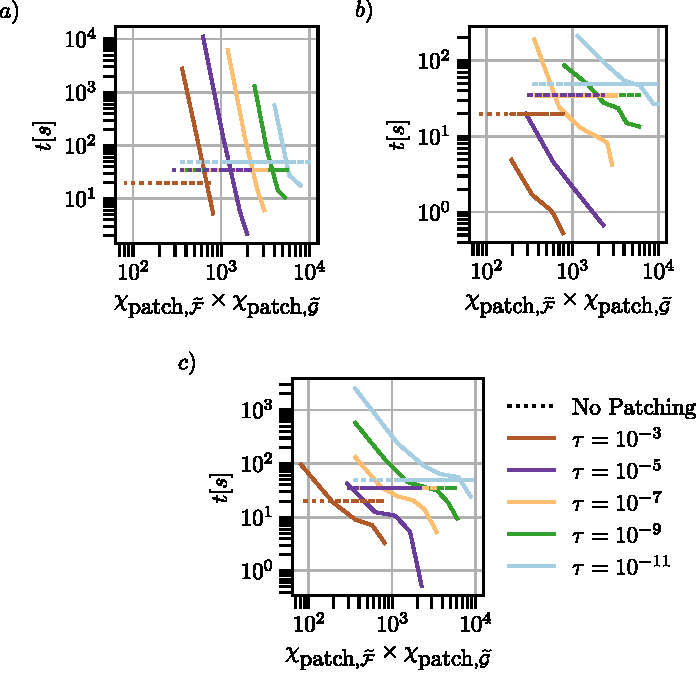
\includegraphics{figures/patchedMulResults.pdf}
    \caption{ Run-time scaling of the patched MPO–MPO contraction for the $(a)$ worst,
    $(b)$ best, and $(c)$ mixed (average) patch arrangements as in \prettyref{fig:patchingPatternsMatMul}. Dotted lines mark the reference time of a monolithic contraction with the same tolerance. }
    \label{fig:patchedMulResults}
\end{figure}

Key observations:

\begin{itemize}
    \item \emph{Worst-case layout}—column patches on both factors—exhibits the slowest scaling, consistent with the \(\mathcal N_{\text{patch}}^{2}\) contraction count predicted in \prettyref{eq:worsScaling}.
    \item For very small \(\chi_{\text{patch}}\) all three patch configurations rise again, signalling \emph{over-patching}: the initial pQTCI step subdivides \(\mF\) and \(\mG\) so aggressively that the overhead of launching thousands of tiny contractions outweighs the benefit of lower ranks.
    \item Around an intermediate, problem-dependent \(\chi_{\text{patch}}^{\mathrm{opt}}\) the patched approach becomes advantageous.  In the best-case arrangement [panel~(b)] the speed-up reaches an order of magnitude relative to the single-core baseline.
\end{itemize}

The speed-up is consistent with the limits on $\Np$ derived in Eqs~\eqref{eq:worstBound}-\eqref{eq:averageBound}; a detailed analysis is provided in Sec.\ref{sec:PatchContrbounds} of Appendix~\ref{app:bounds}.


\subsection{Element-wise multiplication}

Let \(\mF_{\bsigma}\) and \(\mG_{\bsigma}\) be represented in either the
\emph{interleaved} or \emph{fused} quantics format.  
After pQTCI compression and MPO diagonalisation
(\prettyref{eq:diagSiteTensors}), the two MPOs can be fed to the \emph{patched
element-wise contraction} routine, which produces
\begin{equation}
 \bigl(\mF\mG\bigr)_{\bsigma} = \mF_{\bsigma}\mG_{\bsigma}
 \label{eq:elemMulTensor}
\end{equation} 
i.e.\ the tensorised counterpart of the pointwise product 
\begin{equation}
    (fg)(x,y) = f(x,y)g(x,y).
\end{equation}
Knowing the analytic forms of \(f\) and \(g\), we monitor the patchwise error with the metric of \prettyref{eq:localError2DGreen} (where $\bk \to \bx$).  
\prettyref{fig:localErrorElemmul} shows the local error across the domain for a set tolerance \(\tau=10^{-7}\)—applied both in pQTCI and as the square root of the singular value cutoff threshold in each \emph{zip-up} contraction.

\begin{figure}[htpb]
    \centering
    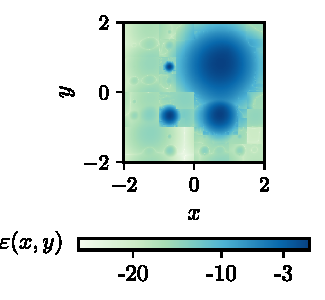
\includegraphics{figures/elemMulError.pdf}
    \caption{Pointwise error \(\varepsilon(\bx)\) of the patched element-wise product for \(\tau=10^{-7}\), $\chi_{\text{patch},\mF} = \chi_{\text{patch},\mG} = 68$ with interleaved ordering.}
    \label{fig:localErrorElemmul}
\end{figure}



Because a diagonal MPO is non-zero only on matching input/output indices, two patches contribute to the product only if they cover the \emph{same} \((x,y)\) tile.  
\prettyref{fig:patchingPatternsElemMul} illustrates this: panels $(a)$ and $(b)$ show the patch layouts of the patched tensors \(\mF\) and
\(\mG\); panel (c) displays the resulting patches of the product, which appear only where the patched in $(a)$ and $(b)$ overlap (cf.\
\prettyref{fig:patchElemContr}). The result is a patched tensor \(\bigl(\mF\mG\bigr)\) that inherits -- in each region of the domain -- the smallest subdivision possible between the two factors.
\begin{figure}[htbp]
    \centering
    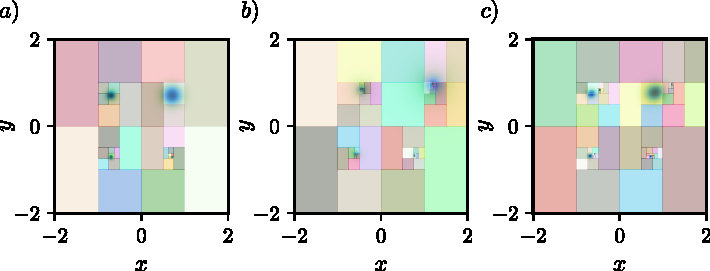
\includegraphics{figures/ElemmulResults.pdf}
    \caption{Patch tilings of $(a)$ \(\mF\), $(b)$ \(\mG\) and $(c)$ their patched element-wise product \(\bigl(\mF\mG\bigr)\). Only overlapping tiles produce a non-zero result.}
    \label{fig:patchingPatternsElemMul}
\end{figure}

Element-wise multiplication enjoys the most relaxed patch-count bound (\prettyref{eq:elemMulBound}; see also
Sec.~\ref{sec:PatchContrbounds} in Appendix~\ref{app:bounds}), and the timing
data in \prettyref{fig:elemMulResults} confirm the advantage. With fused ordering the patched routine achieves up to a five-fold speed-up
over a monolithic contraction; interleaved ordering is still faster than the baseline in for some choices of $\chi_{\text{patch},\mF}$ and $\chi_{\text{patch},\mG}$, though by a smaller margin.



\begin{figure}[ht!]
    \centering
    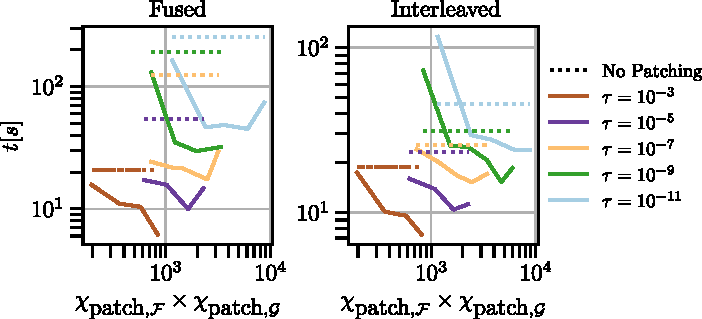
\includegraphics{figures/elemmulTimeResults.pdf}
    \caption{Runtimes for patched element-wise multiplication versus the product of the bond caps \(\chi_{\text{patch},\mF}\times\chi_{\text{patch},\mG}\). Solid lines: patched contraction with fused or interleaved index ordering; dotted lines: reference time for a single, non-patched contraction at the same tolerance. }
    \label{fig:elemMulResults}
\end{figure}

\subsection{Adaptive matrix multiplication}


As a proof of concept for the \emph{adaptive patched MPO–MPO contraction} -- or \textit{adaptive matrix multiplication} -- algorithm we revisit the tensors \(\mF_{\bsigma}\) and \(\mG_{\bsigma}\), now stored in the \emph{fused} quantics ordering.  Suppose we are interested only in a compact representation of
their matrix product $\mathcal H_{\bsigma\bsigma''}$ (cf. \prettyref{eq:matrixMulTensors}) and we \emph{expect} the result to develop sharp, localised structures.
The adaptive workflow proceeds as follows:\footnote{The code used here
incorporates several bug fixes that became available only during the final
stage of writing, thus the limited numerical results.}



\begingroup
\renewcommand{\labelenumi}{(\roman{enumi})}
\begin{enumerate}
  \item Convert \(\mF\) and \(\mG\) to MPS form
        \(\widetilde{\mF}\) and \(\widetilde{\mG}\) using (Q)TCI.
 \item Run the adaptive patched contraction, which recursively slices the two MPOs whenever an intermediate bond exceeds the cap \(\chi_{\text{patch}}\). The procedure stops when every partial product satisfies the target tolerance $\tau$ (see \prettyref{fig:adaptiveMatMul}).
  \item Unfold each resulting patch
        \(\widetilde{\mathcal H}^{p_{1},\dots,p_{\bar\ell}}\) back into an MPS for downstream calculations.
\end{enumerate} 
\endgroup

\prettyref{fig:adaptiveMulResults} demonstrates the outcome. Panel~$(a)$ shows how the adaptive algorithm concentrates patches exactly
where \(\mathcal H\) is most structured, while panel~$(b)$ compares memory requirements with those of a ``naive'' single MPO–MPO contraction.
The feature–aware tiling reduces the parameter count—analogous to the savings pQTCI achieves over standard QTCI for function approximation.
\begin{figure}[ht!]
    \centering
    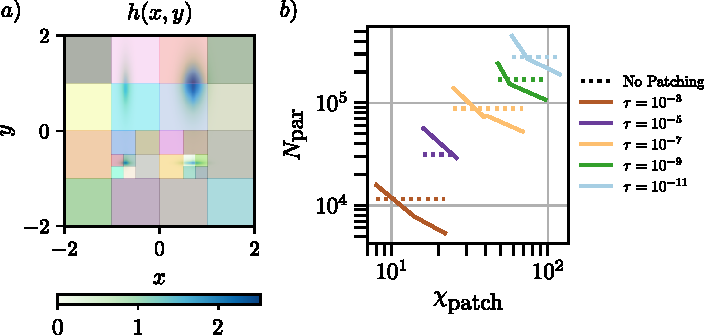
\includegraphics{figures/adaptiveMulResults.pdf}
    \caption{Adaptive patched contraction.
    (a) Patch layout of the product tensor \({\mathcal H}_{\bsigma} = h(\bx(\bsigma))\) obtained by the adaptive contraction algorithm; patches cluster around the high-feature regions.
    (b) Total number of floating-point parameters versus bond–dimension cap \(\chi_{\text{patch}}\). Solid line: adaptive contraction; dotted line: monolithic MPO–MPO multiplication at the same accuracy.}
    \label{fig:adaptiveMulResults}
\end{figure}




\section{Bare Susceptibility Calculation}
\label{sec:bubbleCalc}

We consider now the momentum dependence in the case of the single-orbital Hubbard model on the square lattice at half filling. 
The Hamiltonian of the Hubbard model reads
\begin{equation}
    \mathcal{H} = \sum_{\langle ij \rangle, \sigma} \hat{c}^\dag_{i\sigma}\hat{c}_{\sigma} + U \sum_{i} \hat{n}_{i\uparrow}\hat{n}_{i\downarrow} - \mu\sum_{i,\sigma}\hat{n}_{i\sigma}
    \label{eq:HubbardHamiltonian}
\end{equation}
where $\hat{c}^\dag_{i\sigma}$ is the creation operator of an electron with spin $\sigma$ at site $i$ and $\hat{n}_{i\sigma}=\hat{c}^\dag_{i\sigma}\hat{c}_{i\sigma}$. $U$ is the onsite repulsion and $\mu$ is the chemical potential ($\mu=U/2$ at half filling). The nearest-neighbour hopping is set to one.
In the FLEX approximation \cite{Bickers1989}, for a paramagnetic state the self-energy is approximated as
\begin{equation}
    \Sigma(\bk, i\nu) = \frac{1}{\beta N_{\bk} } \sum_{\bq,i\omega}V(\bq, i\omega) G(\bk - \bq, i\nu - i\omega)
\end{equation}
where $N_{\bk}$ is the size of the two-dimensional momentum grid, $\bq$ is a bosonic momentum, $\nu$ and $\omega$ are Matsubara frequencies, fermionic and bosonic, respectively, and $\beta$ is the inverse of the temperature. The effective interaction is defined as
\begin{equation}
    V(\bq, i\omega) = U^2\left(\frac{3}{2} \chi_{\text{s}}(\bq, i\omega) + \frac{1}{2} \chi_{c}(\bq, i\omega) - \chi_{0}(\bq, i\omega)\right)
\end{equation}
where we introduced the bare $\chi_{0}(\bq, i\omega)$, spin $\chi_{\text{s}}(\bq, i\omega)$ and charge $\chi_{c}(\bq, i\omega)$ susceptibilities. In particular the bare susceptibility reads:
\begin{equation}
    \chi_{0}(\bq, i\omega) = -\frac{1}{N_{\bk}\beta} \sum_{\bk, i\nu} G(\bk + \bq,i\nu + i\omega)G(\bk, i\nu)
    \label{eq:bareSusceptibility}
\end{equation}
where the Green's function in the Matsubara axis is given by 

\begin{equation}
  G(\mathbf{k}, i\nu)
  \;=\;
  \frac{1}
       {\,i\nu+\mu-\varepsilon_{\mathbf{k}}-\Sigma(\bk, i\nu)},
       \label{eq:greenBubble}
\end{equation}
with $\varepsilon_{\bk} = -2 \cos (k_x) - 2 \cos (k_y)$ and $\mu=0$. Hence the bare susceptibility $\chi_{0}(\bq, i\omega)$ is a crucial ingredient in the self-consistent FLEX scheme, where one repeatedly updates the self-energy $\Sigma(\bk, i\nu)$. Therefore, the convolution in \prettyref{eq:bareSusceptibility} quickly becomes the dominant cost, in particular at low temperatures ($\beta \to \infty$). This is because the fermionic Matsubara grid \(\nu_n=(2n+1)\pi/\beta\) grows denser while, at the same time, the Green’s function $G(\mathbf{k}, i\nu)$ develops increasingly sharp, localized peaks (cf. \prettyref{sec:2DGreen}); direct numerical evaluation is both memory- and time-intensive. These characteristics suggest that a domain-adaptive strategy--specifically, the pQTCI-based patched contraction routines introduced above--can alleviate the cost of the convolution by concentrating bond dimension only where the integrand is genuinely singular.

A direct tensor‐train treatment of the convolution in \prettyref{eq:bareSusceptibility} would require handling a six-dimensional integrand-- a challenging task even for QTCI. The remedy is to migrate the calculation to “real” space–time, where the
convolution becomes an \emph{element-wise} product of two functions, after Fourier transform (FT) (cf. Ref.~\cite{Rakhuba2015}).
We define the forward and inverse transforms of the Green’s function as
\begin{align}
     G(\bk, i\nu) &=  \frac{\beta}{\sqrt{N_{\bk}}}\int_{0}^{\beta} d\tau \sum_{\boldsymbol{r}} e^{+\bk\boldsymbol{r}+i\nu\tau}  G(\boldsymbol{r}, \tau) 
     \label{eq:FTGreensFunc} 
     \\
    G(\boldsymbol{r}, \tau) &= \frac{1}{\sqrt{N_{\bk}}\beta}\sum_{\bk,i\nu} e^{-\bk\boldsymbol{r}-i\nu\tau} G(\bk, i\nu) 
    \label{eq:invFTGreensFunc} 
\end{align}
where the sum $\sum_{\nu}$ runs over the Matsubara frequency grid \(\nu_n=(2n+1)\pi/\beta\) with $n=-N_{\nu}/2, -N_{\nu}/2+1, \dots, N_{\nu}/2-1$. 

With these conventions the bare susceptibility reads
\begin{equation}
    \chi_{0}(\bq, i\omega) = \text{FT}\left[ \chi(\boldsymbol{r}, \tau) \right] = \text{FT}\left[ G(\br, \tau)G(-\br, -\tau)\right]
\end{equation}
where  $G(-\br, -\tau)$  is obtained from \prettyref{eq:invFTGreensFunc} by reversing the signs in the exponent. Thus, the six-dimensional convolution is replaced by a pointwise product in $(\br, \tau)$ space -- well suited for the patched element-wise contraction routines introduced earlier.

The complete workflow for evaluating the bare susceptibility \(\chi_{0}(\mathbf q,i\omega)\) is depicted in the flowchart of \prettyref{fig:bubbleFlowchart}.  


\begin{figure}[htbp]
    \centering
    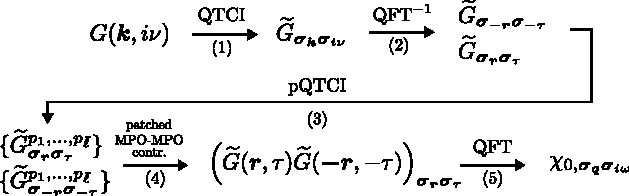
\includegraphics{figures/bubbleFlowchart.pdf}
    \caption{Pipeline for computing the bare susceptibility \(\chi_{0}(\bq,i\omega)\).}
    \label{fig:bubbleFlowchart}
\end{figure}

We proceed through the following stages:

\begingroup
\renewcommand{\labelenumi}{(\arabic{enumi})}
\begin{enumerate}
    \item A QTCI compression of the Green’s function in \prettyref{eq:greenBubble} is performed with the momentum/frequency
    index order \(\bk(\bsigma_{\bk})=\mathbf k(\sigma_{1},\dots,\sigma_{2\mathcal R})\),
    \(i\nu(\bsigma_{i\nu})=i\nu(\sigma_{2\mathcal R+1},\dots,\sigma_{3\mathcal R})\), yielding the TT \(\widetilde G_{\bsigma_{\bk}\bsigma_{i\nu}}\).
    \item The inverse quantics Fourier transform ($\text{QFT}^{-1}$) is applied separately to the \(\bk\) and \(i\nu\) registers, producing the real–space tensors \(\widetilde G_{\bsigma_{\br}\bsigma_{\tau}}\) and \(\widetilde G_{\bsigma_{-\br}\bsigma_{-\tau}}\), with reordered indices \(\br(\bsigma_{\br})=\mathbf r(\sigma_{\mathcal R+1},\dots,\sigma_{3\mathcal R})\)
    and \(\tau(\bsigma_{\tau})=\tau(\sigma_{1},\dots,\sigma_{\mathcal R})\)
    (index reversal is an intrinsic feature of the QFT; see \prettyref{app:QFT}).
    \item Two copies, \(\widetilde G(\mathbf r,\tau)\) and \(\widetilde G(-\mathbf r,-\tau)\), are each patched with pQTCI, by fixing a bond-dimension cap \(\chi_{\text{patch}}\) and a compression tolerance $\tau$. 
    \item The two patch collections are multiplied patch-wise using the patched element-wise contraction routine rendering the product \(\widetilde G(\mathbf r,\tau)\widetilde G(-\mathbf r,-\tau) \)
    \item After summing the patches of the element-wise product into a
    single TT, a direct QFT maps the result back to \((\mathbf q,i\omega)\)
    space, yielding the sought susceptibility
    \(\chi_{0}(\mathbf q,i\omega)\).
\end{enumerate}
\endgroup


In step~(1) we deliberately place the \(\bk\) bits before the \(i\nu\) bits to minimise the intermediate bond dimension of
\(\widetilde G_{\bsigma_{\bk}\bsigma_{i\nu}}\). Because the quantics Fourier transform reverses the bit order within each register (see \prettyref{app:QFT}), the subsequent real-space representation naturally acquires the ordering
\(\mathbf r(\bsigma_{\mathbf r})=\mathbf r(\sigma_{\mathcal R+1},\dots,
  \sigma_{3\mathcal R})\) and
\(\tau(\bsigma_{\tau})=\tau(\sigma_{1},\dots,\sigma_{\mathcal R})\),
after index rearragnement. The rearrangement is performed by inverting the site tensors in real space in order to obtain a sequential index ordering, while conserving the links between the transformed site tensors. Hence, the frequency indices move from the back to the front of the TT in real space. 

Figure \prettyref{fig:heatmapBubble} tracks the steps of the FLEX ``bubble'' $\chi_0$ calculation:
\begingroup
\renewcommand{\labelenumi}{($\alph{enumi}$)}
\begin{enumerate}
    \item  \(\lvert G(\mathbf k,i\pi/\beta)\rvert\) on the Brillouin zone
  \([-\pi,\pi]^{2}\) together with the bond dimension profile of its QTCI representation.
\item Resulting bare susceptibility
  \(\chi_{0}(\mathbf q,\omega\!=\!0)\) and the bond dimensions of its single-TT compression after the final $\text{QFT}^{-1}$.
\item Patch layout produced by pQTCI for the real-space Green’s function \(G(\mathbf r,\tau=\beta)\). Colours indicate distinct patches; correspondent color coding is used for the bond dimensionsof each TT patch, contrasted with those of a global non-patched TT approximation of the real space Green's function.
\end{enumerate}
\endgroup 

The data in \prettyref{fig:heatmapBubble} were obtained with $\mR=13$ bits for each spatial and frequency variable, an inverse
temperature $\beta=100$ , and a uniform accuracy target $\tau=10^{-7}$ (applied to the QTCI and pQTCI compressions and--as $\tau^2$--to the local truncation threshold in every MPO-MPO contraction).

\begin{figure}[htpb]
    \centering 
    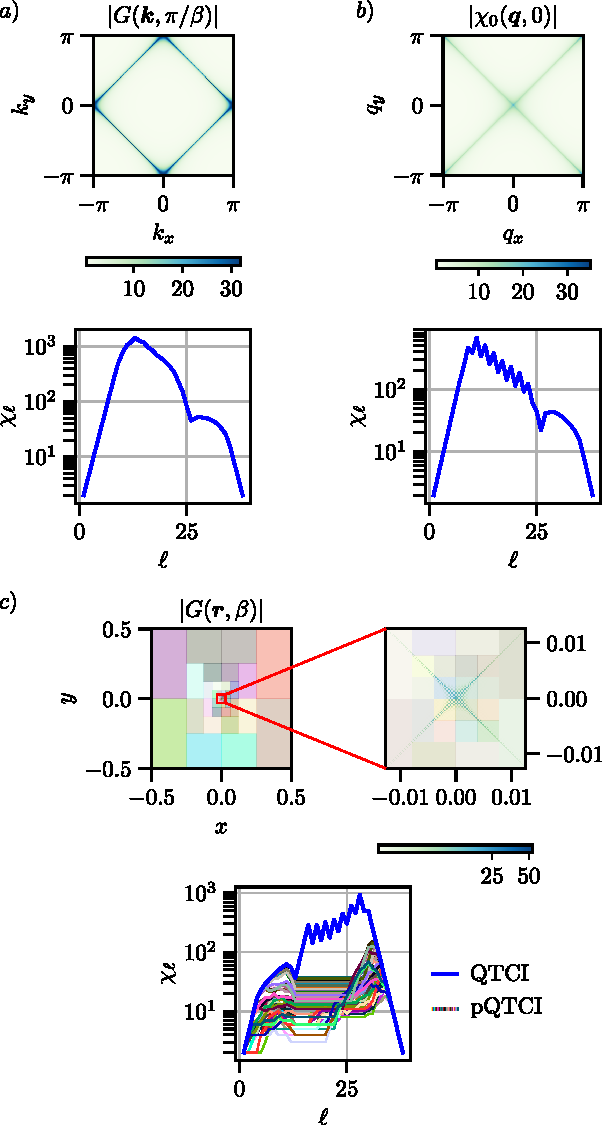
\includegraphics{figures/heatmapBubble.pdf}
    \caption{Heat-map overview of the bare-susceptibility workflow with $\mR=13$, $\beta=100$ and tolerance $\tau=10^{-7}$.
    $(a)$ Absolute value of the Green’s function $G(\bk,i\nu)$ at the first positive fermionic Matsubara frequency, including QTCI bond dimensions 
    $(b)$ Bare susceptibility \(\chi_{0}(\bq,\omega=0)\) with the bond dimensions of its single-TT approximation. 
    $(c)$ Adaptive patching pattern for \(G(\mathbf r,\tau=\beta)\) with bond dimensions profile of each patch and analogous non-patched approximation.}
    \label{fig:heatmapBubble}
\end{figure}

Let us now benchmark the results of the computation. We first verify that the bit-depth chosen for the final calculation, \(\mathcal R=13\), yields a sufficiently converged susceptibility.
Panel $(a)$ of \prettyref{fig:bubbleResults} plots the configuration-space error

\begin{equation}
    \varepsilon(\mathcal R)
  = \frac{1}{\sqrt{N_{\text{err}}}} \sqrt{\sum_{\bsigma_{\bq},\bsigma_{i\omega}} \bigl|
      \chi_{0, \bsigma_{\bq},\bsigma_{i\omega}}^{(\mathcal R,\tau)}
      -\chi_{0, \bsigma_{\bq},\bsigma_{i\omega}}^{(13, 10^{-9})}
    \bigr|^2}
\end{equation}

as a function of $\mR$, for $N_{\text{err}}$ points extracted randomly from the configuration space.  While the curve indicates that \(\chi_{0}\) has not reached the desired precision, the residual error suffices for the present comparative study.

Panel $(b)$ compares the total parameter count of the patched QTCI representation of \(G(\mathbf r,\tau)\) (the same holds for
\(G(-\mathbf r,-\tau)\)) with that of a single-TT QTCI approximation. The patched version saves memory, showing that its patch number respects the theoretical limit
(\prettyref{eq:chiPatchBound}) and, by extension, the element-wise-product bound (\prettyref{eq:elemMulBound}). Hence, we expect an advantage for the patched point-wise contraction. 

Panel $(c)$ reports the wall-clock time on an
Intel\textsuperscript{\textregistered} Xeon\textsuperscript{\textregistered}
E5-2680\,v4 @ 2.40 GHz for the patched element-wise contraction versus the
``naïve'' single-shot contraction, scanned over tolerances \(\tau\) and inverse temperatures \(\beta\). The patched routine accelerates the
calculation by up to an order of magnitude.  For the coldest cases $\beta=100,1000$ the monolithic contraction could not be completed owing to excessive memory demands, whereas the patched algorithm ran comfortably, illustrating the practical benefit of trading one large \(\chi^{4}\) operation for many lower-rank contractions.

\begin{figure}[htpb]
    \centering
    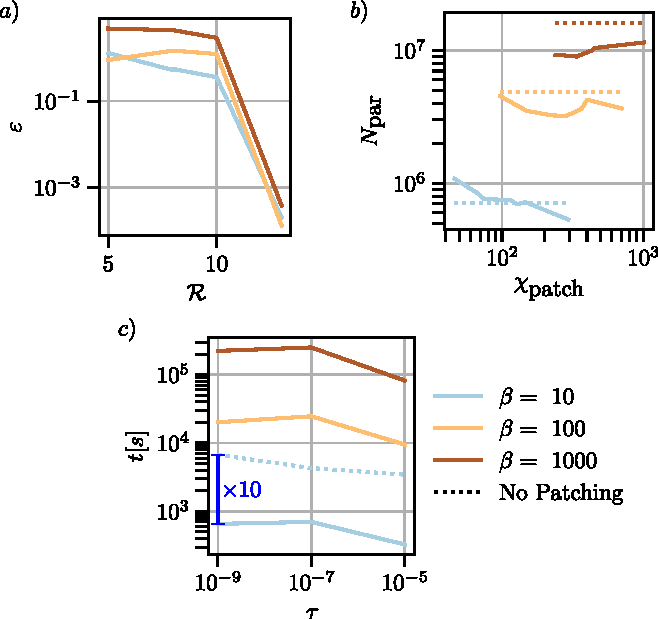
\includegraphics{figures/convergenceBubble.pdf}
    \caption{Performance of the bubble calculation.
    $(a)$ Convergence of \(\chi_{0}\) with bit depth \(\mathcal R\).
    $(b)$ Total number of floating-point parameters in the patched (solid) versus single-TT (dotted lines) representations of \(G(\mathbf r,\tau)\) at \(\tau=10^{-9}\) and $\mR=13$.
    (c) CPU time for the patched element-wise product compared with the monolithic contraction as a function of tolerance \(\tau\) and at different inverse temperatures \(\beta\).}
    \label{fig:bubbleResults}
\end{figure}

\prettyref{fig:betaScaling} tracks the CPU time required for the patched element-wise product as the inverse temperature \(\beta\) is varied
at several accuracy targets \(\tau\).
Within numerical scatter the data follow an \emph{approximately linear} growth, \(t_{\text{CPU}}\propto\beta\) as indicated by the dotted line.

\begin{figure}[htpb]
    \centering
    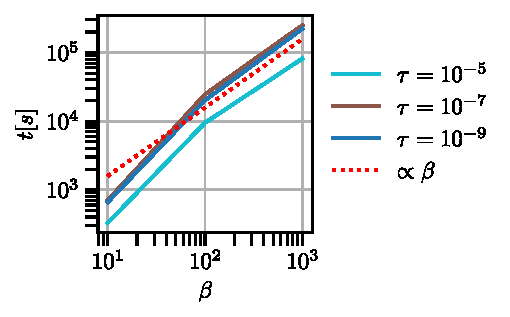
\includegraphics{figures/betaScalingBubble.pdf}
    \caption{Run-time versus inverse temperature \(\beta\) for the patched
    element-wise contraction (solid curves) at three tolerances \(\tau\). Times are measured on an Intel\textsuperscript{\textregistered} Xeon\textsuperscript{\textregistered} E5-2680 v4 @ 2.40 GHz.  The patched algorithm exhibits an almost linear \(\beta\) dependence as highlighted by the fit (dotted curve).}
    \label{fig:betaScaling}
\end{figure}

In this prototype calculation we applied pQTCI and patched contractions \emph{only} to the element-wise multiplication step, which is the dominant bottleneck.
A fully patched treatment of the momentum-space Green’s function \(G(\bk,i\nu)\) would in principle yield an additional speed-up, but was not necessary to demonstrate the merits of the method: even this partial application suppresses the \(\chi^{4}\) scaling, delivers
order-of-magnitude run-time gains, and keeps the memory footprint below that of the traditional approach. These results underline the practicality of the patched QTCI
toolkit for low-temperature perturbative many-body calculations.

\section{Bethe-Salpeter equations with pQTCI} 
\label{sec:patchBSE}
The many-body Hubbard lattice can be reduced to a single, isolated site whose Hamiltonian is
\begin{equation}
    \mathcal{H} = U\hat{n}_{\uparrow}\hat{n}_{\downarrow} - \mu(\hat{n}_{\uparrow} - \hat{n}_{\downarrow})
\end{equation}
where the hopping is naturally set to zero and $\mu$ and $U$ are set to the same values as in \prettyref{eq:HubbardHamiltonian} (half-filling). Despite its simplicity, this \emph{atomic limit} reproduces many key features of the Hubbard model in the strong-coupling regime \cite{Thunstrom2018}.

In the \emph{single–impurity Anderson model} (SIAM) one embeds this single interacting site in a bath of non-interacting electrons. The SIAM Hamiltonian reads \cite{Hewson1993}
\begin{equation}
    \begin{aligned}
    \mathcal{H} &= \sum_{\bk\sigma}\varepsilon_{\bk}\hat{c}^\dag_{\bk\sigma}\hat{c}_{\bk\sigma} + \sum_{\bk\sigma}\left( V_{\bk}\hat{c}^\dag_{\bk\sigma}\hat{d}_{\sigma} + V^*_{\bk}\hat{d}^\dag_{\sigma}\hat{c}_{\bk\sigma}\right) \\ &+ U\hat{n}_{d\uparrow}\hat{n}_{d\downarrow} + \varepsilon_d (\hat{n}_{\uparrow} + \hat{n}_{\downarrow})
        \end{aligned}
\end{equation}
where $\hat{d}^{(\dag)}_{\sigma}$ annihilates (creates) an electron with
spin $\sigma$ in the impurity level $\varepsilon_d=-U/2$, $\hat{n}_{d,\sigma}=\hat{d}^{\dag}_{\sigma}\hat{d}_{\sigma}$, and $V_{\bk}$ hybridises the impurity with the conduction states $\hat{c}^\dag_{\bk\sigma}$, $\hat{c}^\dag_{\bk\sigma}$. The SIAM provides a microscopic description of Kondo physics in heavy-fermion compounds and Kondo insulators, and underlies many dynamical mean-field-theory (DMFT) calculations \cite{Schrieffer1966,Hewson1993, Georges1996}. 

We shall not revisit the physics of the SIAM itself; instead, we focus on the computational bottleneck identified in Ref.~\cite{Rohshap2025} and show how it can be alleviated by our patched contraction scheme.

In the parquet formalism \cite{Rohringer2012} the single–impurity problem is reformulated in terms of coupled two-particle vertex equations. In the particle–hole (\textit{ph}) channel the Bethe–Salpeter equations (BSEs) for the density $(d)$ and magnetic $(m)$ components read
\begin{align}
    F_{d}^{\nu\nu'\omega} &= \Gamma_d^{\nu\nu'\omega} - \frac{1}{\beta^2} \sum_{\nu_1\nu_2} \Gamma_d^{\nu\nu_1\omega}\chi_{0,ph}^{\nu_1\nu_2\omega}F_d^{\nu_2\nu'\omega}
    \label{eq:dBSEs}\\
    F_{m}^{\nu\nu'\omega} &= \Gamma_m^{\nu\nu'\omega} - \frac{1}{\beta^2} \sum_{\nu_1\nu_2} \Gamma_m^{\nu\nu_1\omega}\chi_{0,ph}^{\nu_1\nu_2\omega}F_m^{\nu_2\nu'\omega}.
    \label{eq:mBSEs}
\end{align} 
The right–hand side of each equation is a three-indexed three-tensor contraction that must be evaluated many times during the iterative Parquet loop, and thus dominates the overall cost. Rohshap, Ritter \textit{et al.} \cite{Rohshap2025} solved Eqs.\eqref{eq:dBSEs}–\eqref{eq:mBSEs} with great success using QTCI-based tensor trains. Here we revisit the same contraction but replace the monolithic MPO–MPO multiplication by the \emph{patched} strategy developed in \prettyref{chap:MPOcontr}, expecting further savings from the control of local bond dimensions.

\prettyref{fig:vertexMPStoMPO} sketches the workflow for converting a three–frequency vertex
\(V_{\nu\,\nu'\,\omega}\) (\(\nu,\nu'\) fermionic, \(\omega\) bosonic) into the MPO format required by the MPO-MPO contraction algorithms.
\begingroup
\renewcommand{\labelenumi}{(\alph{enumi})}
\begin{enumerate}
  \item Each Matsubara variable is discretised on a binary grid of \(\mathcal R\) bits. Applying QTCI yields a tensor–train\footnotemark\, \( \widetilde V_{\nu,\nu',\omega}\).
  \item The TT is reshaped into an MPO by
        (i) regrouping fermionic indices according to \prettyref{eq:MPStoMPO}, and
        (ii) ``diagonalising'' bosonic tensor cores as in \prettyref{eq:diagMPOs}.  
        This produces an efficient MPO representation whose structure matches the mixed matrix-multiplication and Hadamard operations in
        the Bethe-Salpeter equations.
  \item For a patched treatment the same sequence is applied \textit{per
        patch}: the global QTCI compression is replaced by pQTCI, and the
        subsequent reshaping steps are local to each patch.
\end{enumerate}
\endgroup
\footnotetext{For brevity we drop the subscript $\sigma$ on all quantics bit strings; the frequency is now written simply as $\nu=(\nu_1,\dots,\nu_{\mR})$ which unambiguously denotes the $\mR$-bit representation of the Matsubara index.}

\begin{figure}[htpb]
    \centering
    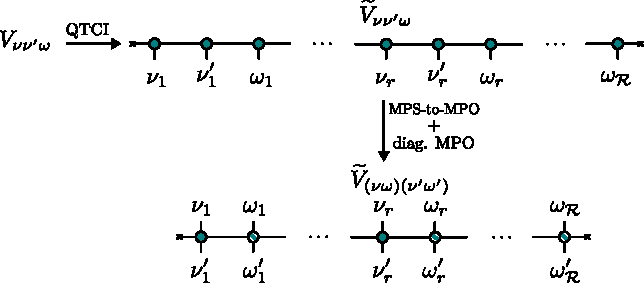
\includegraphics{figures/MPStoMPOVertex.pdf}
    \caption{Transformation of a three-frequency vertex
    \(V_{\nu\,\nu'\,\omega}\) into an MPO: QTCI compression on a \(\mathcal R\)-bit mesh per frequency; TT \(\rightarrow\) MPO mapping via Eqs.~\eqref{eq:MPStoMPO} and~\eqref{eq:diagMPOs}; resulting contraction-ready MPO \(\widetilde V_{(\nu\omega)(\nu'\omega')}\).
    For patched calculations the first step is replaced by pQTCI and the second step is performed on each patch.}
    \label{fig:vertexMPStoMPO}
\end{figure}


The initial stage of the patched BSE scheme is visualised in \prettyref{fig:patchedVertices}.
Using the interleaved slicing order (see
\prettyref{fig:patchingPatternsMatMul}), each two-particle vertex is compressed with pQTCI so that the resulting patch grid adapts to the
structure of the data.
For clarity we display two-dimensional cuts at the bosonic frequency $\omega=0$; the axes correspond to the fermionic frequencies on a $2^{\mR}\times2^{\mR}$ mesh with $\mR = 7$.
The color scale shows $|F_d|$, $|\Gamma_d|$ and $|\chi_{0,ph}|$, respectively, each reconstructed from their patched approximation up to a tolerance $\tau=10^{-7}$. One sees that smaller, tiles concentrate in the regions where the vertices exhibit pronounced structure, whereas featureless areas are covered by larger patches.


\begin{figure}[htpb]
    \centering
    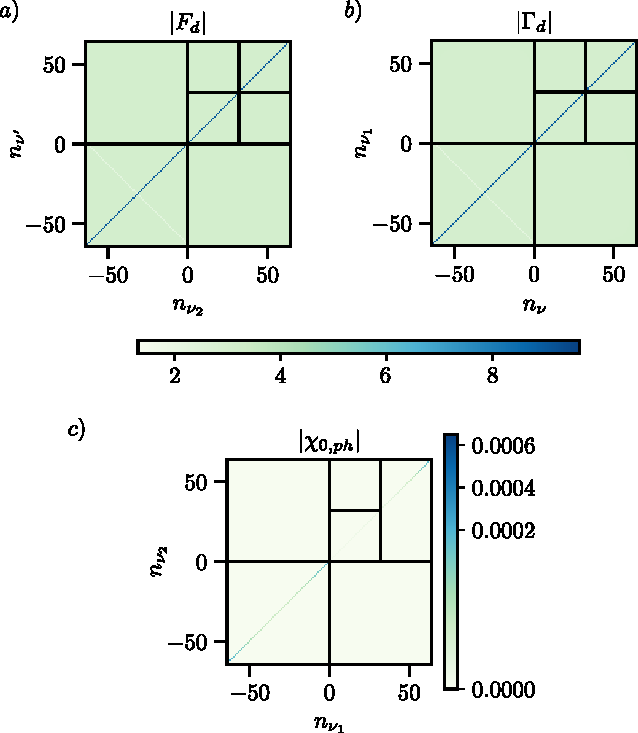
\includegraphics{figures/patchedVertices.pdf}
    \caption{pQTCI compression of the Bethe-Salpeter vertices at $\omega=0$. Panels show $|F_d|$ $(a)$, $|\Gamma_d|$ $(b)$ and $|\chi_{0,ph}|$ $(c)$ on the respective $(\nu_2,\nu')$, $(\nu_1,\nu)$ and $(\nu_2,\nu_1)$ grids for $\mR=7$ and tolerance $\tau=10^{-7}$. Patch boundaries reveal how the adaptive slicing refines only those regions where the vertex is more interesting, also for three dimensional objects.}
    \label{fig:patchedVertices}
\end{figure}

\prettyref{fig:BSEresult} compares the wall-clock time required to evaluate the contraction on the right-hand side of the BSEs with and without patching.  
Calculations were performed on an
Intel\textsuperscript{\textregistered} Xeon\textsuperscript{\textregistered}
E5-2680 v4 @ 2.40 GHz; the horizontal axis shows the number of bits \(\mathcal R\) used per fermionic frequency (i.e.\ \(\mathcal R=\log_{2}N_{\nu}\) with $N_{\nu}$ total frequencies). Four target tolerances \(\tau\) are reported.  
Over the entire range the patched algorithm outperforms the conventional single-MPO contraction by up to an order of magnitude.  
For the stringent tolerance \(\tau=10^{-10}\) the monolithic approach was no longer feasible beyond \(\mathcal R=7\) owing to excessive memory requirements, whereas the patched routine remained tractable.


\begin{figure}[ht!]
    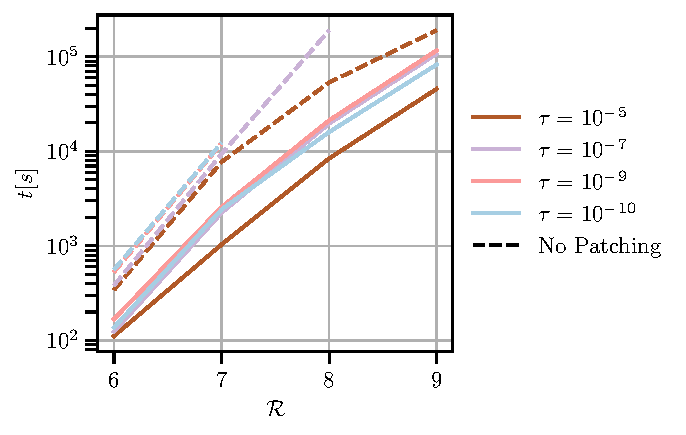
\includegraphics{figures/BSEContraction_R_vs_time_comparTCI.pdf}
    \caption{CPU time for the BSE vertex contraction versus the frequency resolution
    \(\mathcal R\) (bits per Matsubara axis).
    Solid curves: patched MPO–MPO contraction;
    dashed curves: conventional (non-patched) contraction. Colours denote the compression tolerance \(\tau\).}
    \label{fig:BSEresult}
\end{figure}

By decomposing the three-index vertex product into many low-rank patch contractions, the patched MPO strategy removes the \(\chi^{4}\) bottleneck that plagues the standard approach.  
The resulting speed-up highlights the potential of patched tensor-network techniques for
self-consistent parquet calculations at high frequency resolution.

% \section{Gaussian Orbital Overlap}

% \note{Orbitals overlap}{Yuriel's paper on atomic bases: \cite{Jolly2024}, double-zeta calculation(?)}

% The electron repulsion integral of two GTOs is defined as

% \begin{equation}
%     \bra{\textbf{A}, \textbf{C}}\frac{1}{r_{12}}\ket{\textbf{B}, \textbf{D}} = \int_{-\infty}^\infty \text{d}^3r_1 \int_{-\infty}^\infty \text{d}^3r_2 \frac{\phi_\textbf{A}(\bm{r}_1) \phi_\textbf{B}(\bm{r}_1) \phi_\textbf{C}(\bm{r}_2) \phi_\textbf{D}(\bm{r}_2)}{|\bm{r}_1 - \bm{r}_2|}
% \end{equation}

% where the generic Cartedisan GTO can be written as

% \begin{equation}
%     \ket{\textbf{R}} = \phi_\textbf{R}(\bm{r}) = N (x - R_x)^l (y - R_y)^m (z - R_z)^n e^{-\alpha (\bm{r} - \textbf{R})^2}.
% \end{equation}
% The electron repulsion integral can be rewritten as (cf. Ref. \cite{Petersson2010}): 

% \begin{align}
%     \bra{\textbf{A}, \textbf{C}}\frac{1}{r_{12}}\ket{\textbf{B}, \textbf{D}} =& \frac{N_\textbf{A}N_\textbf{B}N_\textbf{C}N_\textbf{D} \pi^{5/2}}{\gamma_p\gamma_q\sqrt{\gamma_p + \gamma_q}} e^{\eta_p(\textbf{A} - \textbf{B})^2} e^{\eta_q(\textbf{C} - \textbf{D})^2} \times \\
%     \nonumber &\sum_{\bm{i},\bm{o},\bm{r},u}\mathcal{J}_x \sum_{\bm{j},\bm{p},\bm{s},v} \mathcal{J}_y \sum_{\bm{k},\bm{q},\bm{t},w} \mathcal{J}_z\ 2F_\nu (\eta (\textbf{P} - \textbf{Q})^2)
% \end{align}

% where

% \begin{equation} 
%     F_\nu(u) = \int_{0}^{1} \text{d}t\ t^{2\nu} e ^{-ut^2}
% \end{equation}

% is the so-called \textit{Boys function} \cite{Boys1950}.

    
% \begin{equation}
%     \begin{alignedat}{5}      
%       \textbf{P} &= \frac{1}{\gamma_p}(\alpha_1 \textbf{A} + \alpha_2 \textbf{B}) &\qquad \gamma_p &= \alpha_1 + \alpha_2 \\[6pt]
%       \textbf{Q} &= \frac{1}{\gamma_q}(\alpha_3 \textbf{C} + \alpha_4 \textbf{D}) &\qquad \gamma_q &= \alpha_3 + \alpha_4 \\[6pt]
%       \eta &= \frac{\gamma_p\gamma_q}{\gamma_p + \gamma_q}
%     \end{alignedat}
% \end{equation}
    

% \begin{figure}[ht!]
%     \caption{TCI and patched TCI approximation of the Boys function.}
% \end{figure}

% \begin{figure}[ht!]
%     \caption{3D graph of Gaussian orbitals for \ce{H2} and \ce{LiH}}
% \end{figure}

% \begin{figure}[ht!]
%     \caption{Memory and time scaling of orbital overlap compared with standard approach. }
% \end{figure}


